\chapter{Systemanalyse}\label{sec:simulation}
Nachdem nun im vorherigen Kapitel ein erstes Modell mitsamt Aktuatorik entwurfen wurde, soll nun überprüft werden, ob dieses unter Last zum einen genügend Festigkeit besitzt und zum anderen, ob die Aktuatorik auch die entsprechenden Leistungen liefern kann. Auf Basis dieser Analysen werden anschließend Optimierungen der in Kapitel \ref{sec:modellentwurf} getroffenen Entscheidungen vorgenommen.


\section{FEM-Analyse}
Solid Edge bietet direkt das integrierte FEM-Program "NX Nastran" an, was einen schnellen Designzyklus von berechnen und Modell bearbeiten ermöglicht. Für eine effiziente FEM-Analyse werden die Modellvarianten zunächst vereinfacht, indem die Verrundungen und Anschrägungen der Wände entfernt werden. Auch einige der steilen Spitzen der Pfeilung werden abgerundet, da diese bei der Vernetzung nur zu Problemen führt und die Belastungen im Material so gut wie gar nicht verändern.

Bevor dir Kräfte aus Formel \ref{eq_Fmax} und \ref{eq_Fmax2} auf die Geometrie angewandt werden können, müssen sie noch aus dem körperfesten in ein Grid Fin festes Koordinatensystem übertragen werden. Dieses ist in Abbildung \ref{abb_gitter} dargestellt und wurde so definiert, dass die Kräfte $F_2$ und $F_3$ genau normal auf den Gitterwänden stehen, sodass sie sich einfach in der FEM-Analyse implementieren lassen. $F_1$ ist parallel zur Sehne und kann somit, genau wie die anderen beiden Kräfte, gleichmäßig auf alle Flächen verteilt werden, die eine Normale haben, die zum Teil in diese Richtung zeigt.
\begin{figure}[h] 
	\centering
	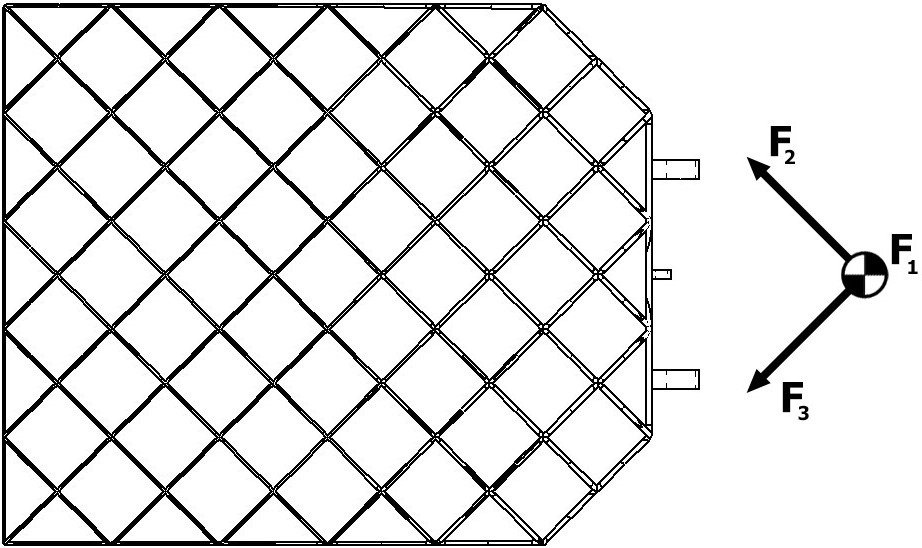
\includegraphics[width=0.9\textwidth]{Gitter.jpg}
	\caption{Kräfte im Grid Fin festen Koordinatensystem}
	\label{abb_gitter}
\end{figure}\\
Somit ergeben sich die Kräfte für die einzelnen Grid Fins zu:
\begin{table}[h]
	\centering
	\begin{tabular}{c||c|c|c|c}
		&D1&R1&D2&R2\\
		\hline
		$F_1/$N&$413,5$&$389,3$&$389,3$&$413,5$\\
		$F_2/$N&$6276,0$&$4970,8$&$-4970,8$&$-6276,0$\\
		$F_3/$N&$4934,0$&$6474,2$&$-6474,2$&$-4934,0$\\
	\end{tabular}
\end{table}
Als Randbedingung werden die Innenflächen der Halterung zylindrisch festgelegt. Das heißt die dort liegenden Knoten können sich weder axial noch radial bewegen, jedoch um die Achse drehen.
\subsection{Optimierung der Halterung}
Bei beiden Pfeilungstypen lässt sich für alle Lastfälle sofort erkennen, dass es zu massiven Lastspitzen an der Halterung kommt. Währenddessen bleiben die Werte im Gitter deutlich niedriger. Der Grund für die hohen Spannungen an der Einspannung ist die ungünstige Lage in der Mitte der Wände anstatt der Schnittstellen, Somit bilden sich vergleichsweise hohe Biegemomente in den Wänden aus. Dieser ungünstige Kraftfluss wird durch die scharfen Kanten weiter verschlimmert. Um nun diese Spannungsspitzen zu vermeiden, sollte, neben einer Abrundung der Kanten, die Position der Halterungen verändert werden.
\begin{figure}[h] 
	\centering
	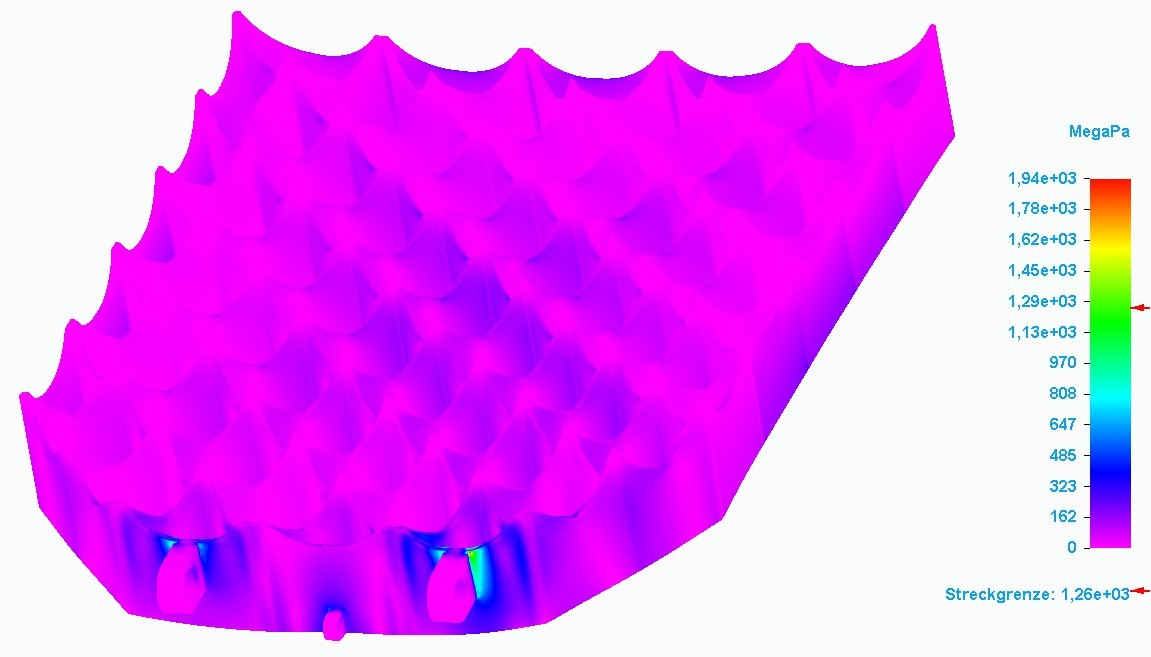
\includegraphics[width=0.9\textwidth]{D1 3.3b max 1.jpg}
	\caption{Maximale Spannungen am Grid Fin D1}
\end{figure}\\
Da sich die Anbringung der Halterungen genau ein der Mitte Zelle befinden, auch wenn sie in diesem Fall halbiert sind, lassen sie sich entweder tangential oder normal zum Raketenkörper verschieben, um sie auf einen Schnittpunkt der Wände zu legen. Soll Halterung B nicht in zwei Teile aufgeteilt werden, so kommt nur eine Bewegung senkrecht zum Körper in Frage. Anstatt die Halterung nun in das Gitter hinein zu legen, was zu einer Verkleinerung der durschdtrömten Querschnittfläche führen würde und somit geringer Normalkräfte, werden zwei der Wände weiter fortgesetzt. Diese schneiden sich dann in der Mitte, wo die Halterung B platziert wird. Die Halterung wird jedoch nicht direkt an der Schnittstelle konstruiert, sondern noch ein bisschen weiter vom Gitter entfernt, sodass die Kraft gradliniger über die Beiden Hubstangen geleitet werden kann.

Für die Halterungen A passiert das gleiche. Die nebenliegenden Gitterwänder werden bis zu ihrer Schnittstelle fortgesetzt. Im Gegensatz zur Halterung B befindet sich jedoch direkt hier die Bohrung, an der das Grid Fin montiert werden soll.
\begin{figure}[h]
	\begin{minipage}[t]{0.45\linewidth}
		\centering
		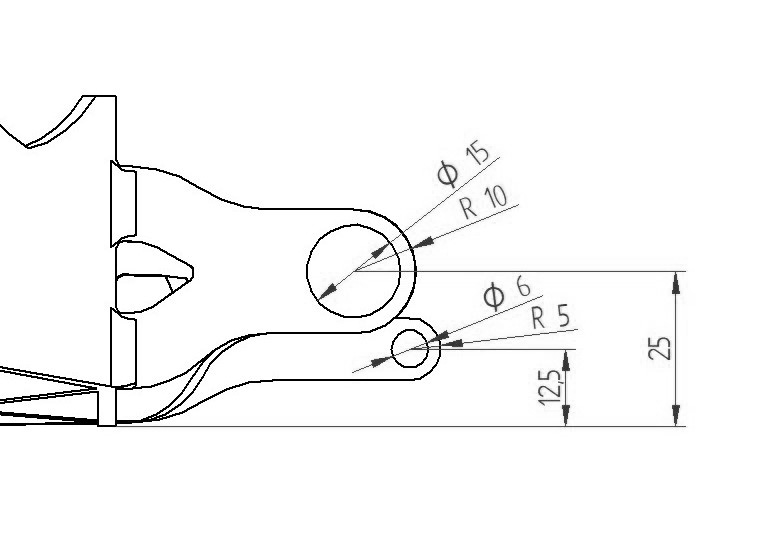
\includegraphics[width=0.85\textwidth]{Skizze Halterung 2.0 1.jpg}
	\end{minipage}
	\hfill
	\begin{minipage}[t]{0.45\linewidth}
		\centering
		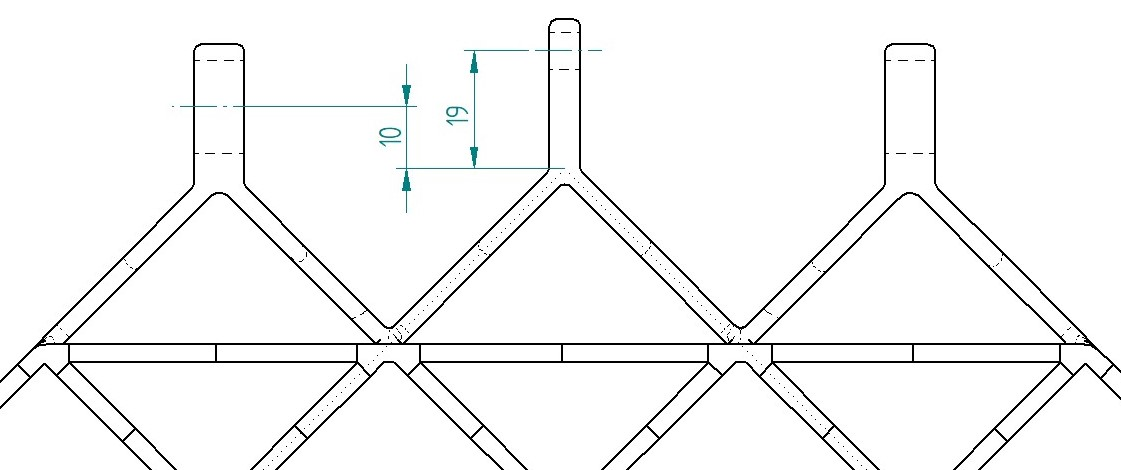
\includegraphics[width=1\textwidth]{Skizze Halterung 2.0 2.jpg}
	\end{minipage}
	\caption{Verbesserte Version der Halterung (1)}
\end{figure}\\
Dies sorgt zwar schon für eine deutlichere Verbesserung, jedoch ist der Hebelarm trotz der Versetzung der Halterung B recht kurz. Dies sorgt dafür, dass dort direkt an der Bohrung noch immer Spannungsspitzen auftreten, die die Streckgrenze von $R_{p, 0.2} = 1262$MPa unterschreiten.
\begin{figure}[h] 
	\centering
	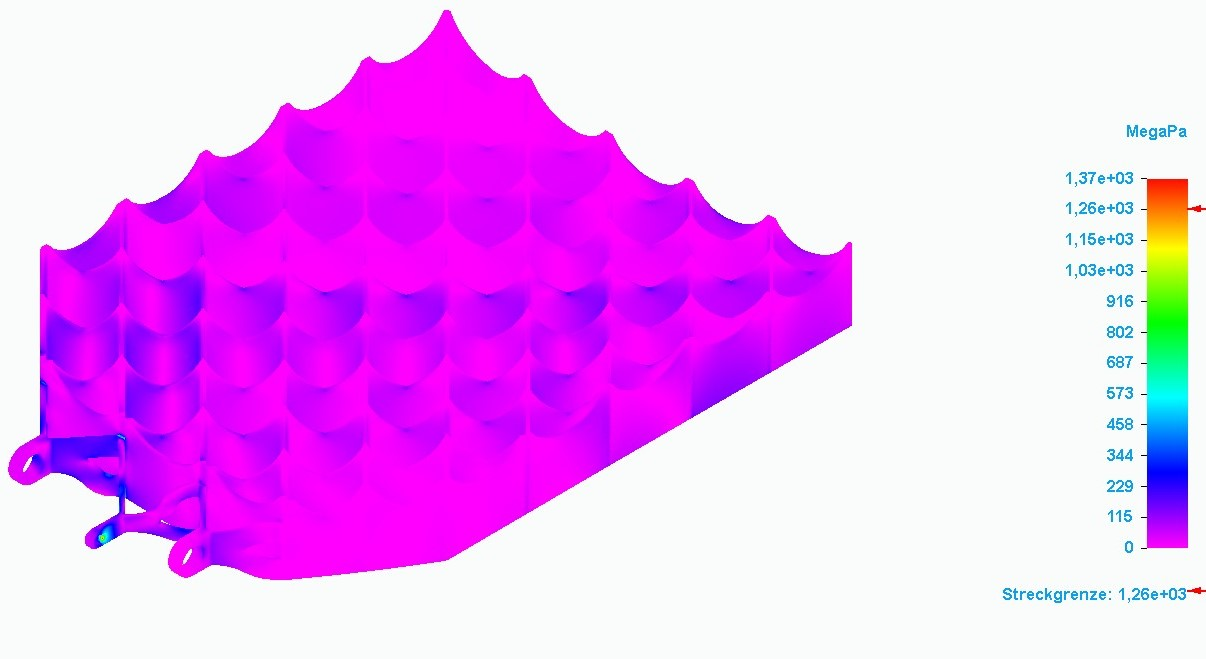
\includegraphics[width=0.9\textwidth]{D2 3.4 b max.jpg}
	\caption{Maximale Spannungen am Grid Fin D2 bei veränderter Halterung(1)}
\end{figure}\\
Um dem Hebelarm zu Verlängern wird nun die Halterung B auf die Höhe der konvexen Seite gebracht. Sie wird außerdem in einer geschwungen Form noch weiter nach vorne gelegt, damit die Verbindungslinie der beiden Halterungen im $45^\circ$ Winkel zur Gitterebene liegt. Dadurch ist die Klappbewegung möglichst gleichmäßig, was den Aktuator schont und gleichzeitig garantiert, dass der Verfahrweg minimal für den gegeben Hebelarm ist.
\begin{figure}[h] 
	\centering
	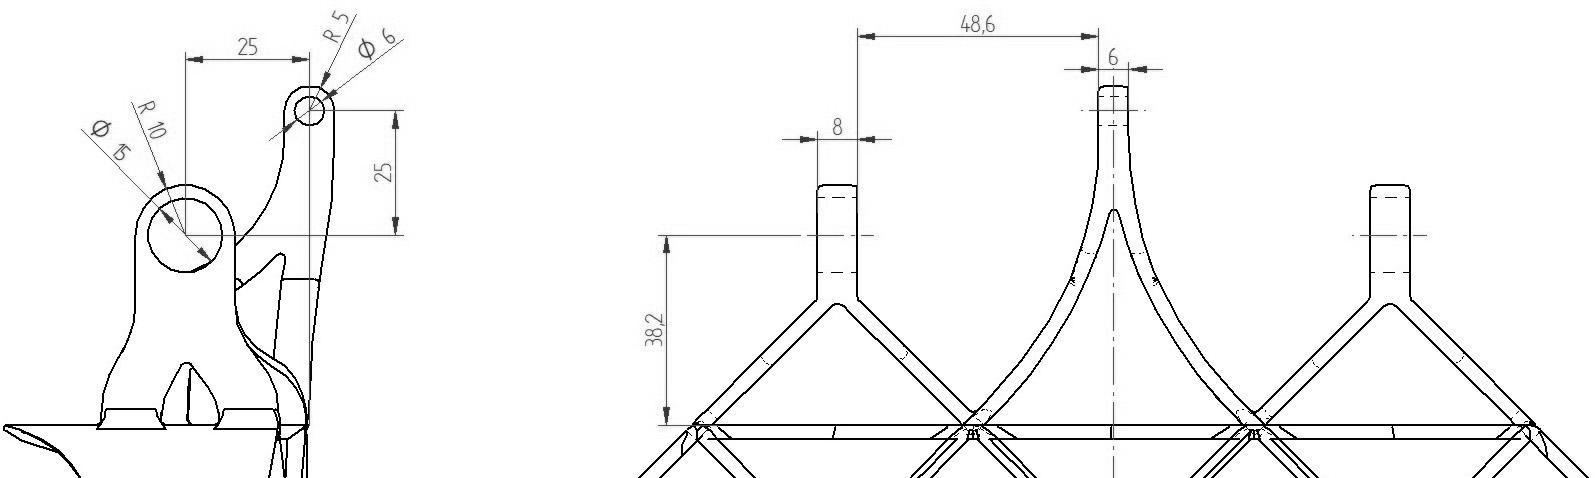
\includegraphics[width=0.9\textwidth]{Skizze Halterung 3.5.jpg}
	\caption{Verbesserte Version der Halterung (2)}
\end{figure}\\
Dies hat nun endlich den gewünschten Effekt, dass die Spannung im Material deutlich niedriger werden. Bei allen Grid Fins treten nur noch Spannungen auf die deutlich unter der Streckgrenze des Materials liegen und somit den Belastungen im Einsatz standhalten.
\begin{figure}[h] 
	\centering
	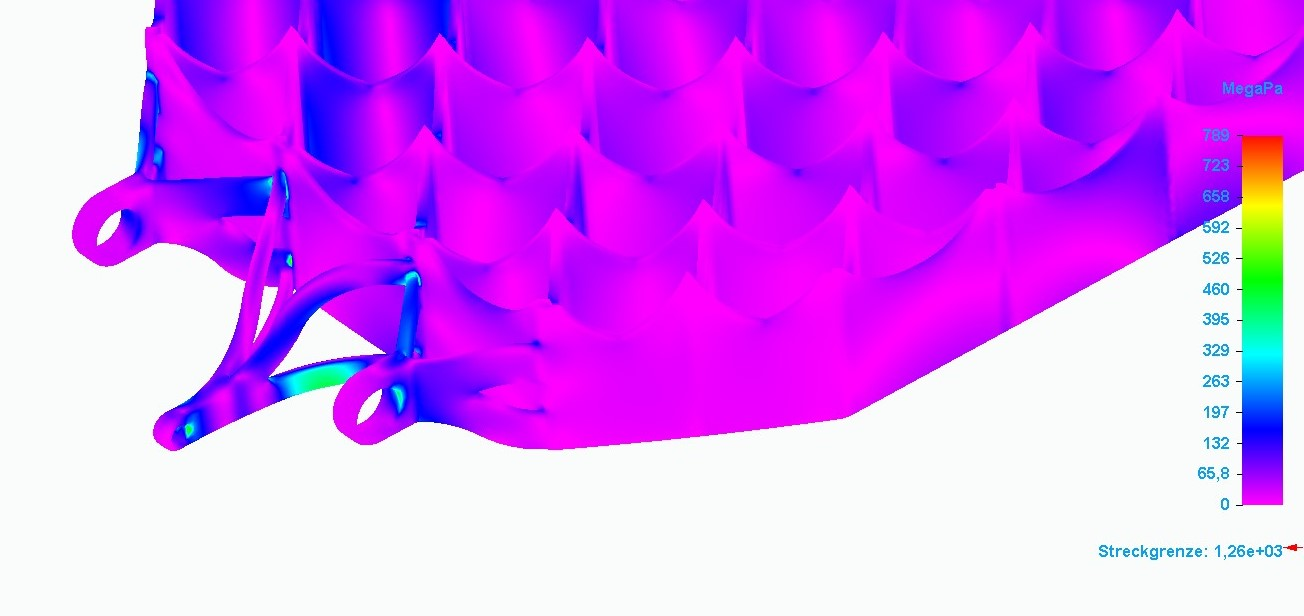
\includegraphics[width=0.9\textwidth]{3.5 b Halterung max.jpg}
	\caption{Maximale Spannungen am Grid Fin D2 bei veränderter Halterung (2)}
\end{figure}\\
Somit wäre die Auslegung der Halterung nach den aerodynamischen Kräften theoretisch abgeschlossen, jedoch muss hierbei auch noch auf die Aktuatorik und das maximale Lastenvielfache geachtet werden. Aktuell hat der Grid Fin eine Masse von $m = 3,5$kg und der Massenschwerpunkt liegt $185$mm von der Halterung A entfernt. Mit dem Lastenvielfachen von ca. 20 beim auslösen des Ballutes entsteht nun also ein Moment von ungefähr $M=127Nm$, welches von der Halterung B kompensiert werden muss. Die Halterung B ist an der Spindelstange montiert und leitet somit die Kraft an diese weiter. Der Hebelarm der Halterung B und die maximale ertragbare Axialkraft der Spindel müssen also aufeinander abgestimmt sein. Maxon Motoren stellt nur Spindeln mit Axiallasten von bis zu $2700$N her, welche folglich einen Hebelarm von $\frac{127Nm}{2700N}=47mm$ erfordert, was noch gerade so für den Grid Fin annehmbar ist. Der Wert liegt laut dieser Rechnung zwar minimal drüber jedoch wird das Lastenvielfache von 20 gar nicht wirklich erreicht, sodass die Rundung annehmbar ist. Da die Hubstange gelenkig mit dem Grid Fin verbunden ist, ist zu beachten, dass nur der Abstand der Haltungen in Sehnenlänge als effektiver Hebelarm wirkt. Somit muss die Halterung B nicht länger weiter vorne positioniert sein, was Material spart. Wird die Verbindungsstange zwischen Halterung und Hubstange auf die gleiche Länge wie der Hebelarm gesetzt, verlängert sich auch nicht der Hub und da die Hubstange nun weiter außerhalb der Rakete im eingeklappten Zustand befindet, braucht sie auch weniger Platz innerhalb der Rakete, wenn der Grid Fin ausklappt. Um auf den gewünschten Hebelarm zu kommen werden nun beide Halterungen noch ein wenig nach außen gelegt, sodass sich die endhültige Geometrie, wie sie in Abbildung \ref{abb_Halterung-fertig} zu sehen ist, ergibt.
\begin{figure}[h] 
	\centering
	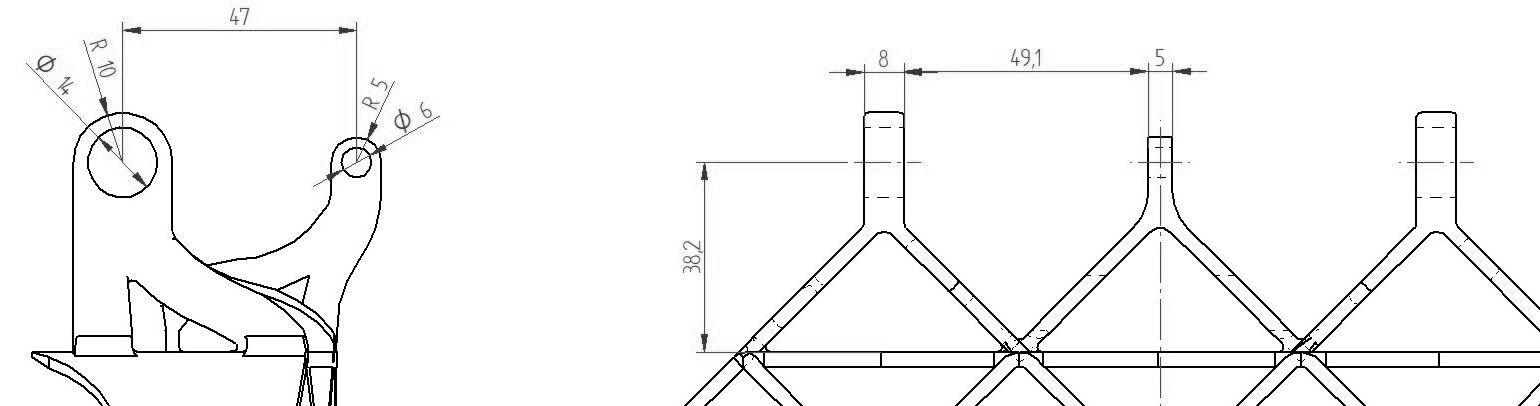
\includegraphics[width=0.9\textwidth]{Skizze Halterung 3.6.jpg}
	\caption{Endgültige Geometrie der Halterung}
	\label{abb_Halterung-fertig}
\end{figure}\\
Zur Bestätigung werden wieder FEM Analysen durchgeführt und diesmal werden ergänzend zu den aerodynamischen Kräften auch in einem separaten Lastfall die Beschleunigungskräfte untersucht. Bei den Lastvielfachen werden die anderen Kräfte ignoriert, da sie eher eine Stützwirkung habe und somit die Spannungen nur weiter senken würde. Beim Auftreten der Ruckartigen Abbremsung durch den Ballonschirm ist der Max Q sowieso schon überschritten uns somit die anderen Kräfte nur noch deutlich geringer. Wie Abbildungen QQQQQQQQQQQQQQ und AAAAAAAAA zeigen wird die Streckgrenze weiterhin nicht unterschritten. Somit gibt die Halterung als bestätigt.
\subsection{Optimierung des Gitters}
Als nächstes wird das Gitter untersucht. Es ist sofort erkenntlich, dass die Belastungen überall relativ niedrig, deutlich unter der Streckgrenze, liegen. Egal ob beim Tal- oder Berg-Typus, die Spannungsspitzen, die auftreten, sind keines Wegs kritisch. Somit ist eine Aufdickung des Material nicht nötig, sondern es kann über eine Reduzierung der Wandstärke nachgedacht werden.

Die Wanddicke ist jedoch nicht nur durch die mechanische Belastung, sondern auch die thermische, nach unten hin beschränkt. Diese ist jedoch ein sehr komplexes Phänomen, das von der Zusammensetzung der Atmosphäre, den zeitlich ändernden Strömungsbedingungen, die Postion des Verdichtungsstoßes und dem Aufbau des Grid Fins abhängen, sodass es nicht auch nur überschlägig in dieser Arbeit behandelt werden kann.
\\~\\
Der Grid Fin ist momentan am von der Rakete weg zeigenden Ende schon nur $1,5$mm dick, was für den Wiedereintritt schon ein relativ kleiner Wert sein könnte. Deswegen soll dieser zunächst nicht unterschritten werden.



~\\~\\
Der Vergleich von der Berg- und Tal-Konfiguration zeigt, 


\section{Bestätigung der Akuatorik}
Nun da die Geometrie des Grid Fins, insbesondere der Halterung fest steht, kann überprüft werden, ob diese der mechanischen Last stand hält. Hierfür werden die Kräfte, die an den einzelnen Halterungen wirken benötigt. Die detaillierte Rechnung befindet sich im Anhang \ref{sec_halterkraefte}. Wenn angenommen wird, dass die Halterung B, da sie deutlich weniger steif als die Halterungen A sind, nur Belastung in $\eta$-Richtung aufnehmen kann ergeben sich die Kräfte wie folgt. Links sind Kräfte am Grid Fin R1 dargestellt, was die höchste Belastung für das Lager A bedeutet, und rechts R2 mit der höchsten Belastung für Lager B.
\begin{table}[h] 
	\centering 
	\begin{tabular}{c|c|c|cc||c|c|c|c} 
		\textbf{R1}&$F_{\zeta}$[N]&$F_\eta$[N]&$F_\xi$[N]&&\textbf{R2}&$F_{\zeta}$[N]&$F_\eta$[N]&$F_\xi$[N]\\ 
		\hline 
		A1& 612,00&-5601,54&-531,55&&A1&599,90&5,16&-474,45\\
		A2&-1001,31&-1624,49&-531,54&&A2&.1013,41&3554,87&-474,45\\
		B&0&-886,81&0&&B&0&4366,53&0\\
	\end{tabular}
\end{table} \\
Für die Lasten an den Lagern ist nur die Aufteilung in Radial- $F_r$ und Axialkraft $F_a$ von Bedeutung. Dabei sei noch zu bedenken, dass die Kraft in $\xi$-Richtung auf Grund des Aufbaus nur von einem der A Lager kompensiert werden kann. Auch wenn das für die vorherige Berechnung keine Rolle spielte, da die beiden Halterungen A auf einer Achse liegen, wird es im folgenden berücksichtigt.
\begin{table}[h] 
	\centering 
	\begin{tabular}{c|c|cc||c|c|c} 
		\textbf{R1}&$F_{r}$[N]&$F_a$[N]&&\textbf{R2}&$F_{a}$[N]&$F_r$[N]\\ 
		\hline 
		A1& 5634,87&-1063,10&&A1&599,92&948,90\\
		A2&1908,29&0&&A2&3696,60&0\\
		B&866,81&0&&B&4366,53&0\\
	\end{tabular}
\end{table} \\
Aus diesen Werten lässt sich nun über die Flächenpressung und Abscherung den erforderlichen Durchmesser $D$ und die benötigte Auflagebreite $B$ der Hilfswelle bestimmen. Für die Abscherung git
\begin{equation}
	\tau_{\mathrm{zul.}}\leq\tau_\mathrm{scher}=\frac{F_r}{m\pi D^2/4}.
\end{equation}
Mit $\tau_{\mathrm{zul.}}=R_{p, 0.2}\cdot 0,6$ \cite{metall} und $m$ als die Anzahl der Schnittflächen lässt sich der Mindestdurchmesser bestimmen.
\begin{equation}
	D \leq \sqrt{\frac{4F}{m\pi 0,6 R_{p, 0.2}}}= 5,5\mathrm{mm}
\end{equation}
Für die Halterung A ist $m=1$, sodass eine Mindestdicke von $D=5,5$mm benötigt wird. Aus der sich eine Auflagebreite von $B = 3,1$mm ergibt. Da sich der Aufbau des Grid Fins seit dem ersten Modell verändert hat, kann auch die Anbringung an der Welle, welche in Abbildung \ref{abb_Welle} zu sehen war, angepasst werden. Durch wie Verlegung der Halterung A rückt der Grid Fin näher an den Raketenkörper ran. Statt nun Greifarme aus der Welle raus ragen zu lassen, wir diese nur ein wenig verlängert, sodass die Verbindungslinie durch die beiden Halterungen A die Welle durchstößt. Auf diese Verbindungslinie wird eine Stange gelegt, auf der der Grid Fin montiert wird. Diese Variante der Halterung hat zum einen den Vorteil, dass keine komplizierte Greiferstruktur gefertigt werden muss, und zum anderen steht nun ein Großteil der planaren Wand im eingeklappten Zustand nicht mehr direkt in der Strömung, sondern im Windschatten der Welle. Dadurch wird ungewollter Widerstand und Belastung der Grid Fins verhindert. Um den Grid Fin reibungsarm zu sicher, muss er sowohl axial als auch radial mit Wälzlagern gelagert werden. Zylinderrollenlager, wie sie auch bei der Welle verwendet werden, sind hier jedoch eine ungünstige Wahl, da sie recht großen Bauraum benötigen. Stattdessen wird die Halterung A auf beiden Seiten mit einem schmalen Nadellager radial und mit einem Kugellager axial mit der Welle verbunden. Diese Kombinationslager werden von außen mit Nutmuttern, die auf die Verbindungsstange aufgeschraubt und durch Sicherungsbleche gesichert werden, an den Grid Fin gedrückt. Um ein Verrutschen der Verbindungsstange in der Welle zu verhindern, muss diese noch durch eine Passschraube fixiert werden. Für diese Passschraube werden wieder aus der Flächenpresssung und der Abscherung die Mindestmaße des Durchmessers und der Breite bestimmt. Mit eim Durchmesser von $D = \mathrm{mm}\gg 1,2$mm und einer Kontaktbreite von $B = \mathrm{mm}\gg 1,3$mm ist sie für diese Anwendung ausreichend.

SKIZZEEEEEEEEEEEEEEEEEEEEE mit Maßen

Die Halterung B wird von beiden Seiten gestützt, sodass mit $m = 2$ ein Mindestdurchmesser von $D = 3,4$mm errechnet wird. Die zugehörige Breite beläuft sich somit auf $B = 3,8$mm. Wie schon angemerkt treten hier kaum Axialkräfte auf, sodass ein Rillenkugellager ausreicht, um diese aufzunehmen. Es wird auf der einen Seite gegen eine Schulter in der Halterung B des Grid Fins gedrückt und auf der anderen Seite durch ein Sicherungsring fixiert. Zwei Stifte werden von beiden Seiten gegen die innere Kante des Lagers gedrückt und miteinander schraubt. Diese Stifte können anschließend von außen mit Muttern an die Verbindungsstange für den Hub fixiert werden. Somit ist auch die Halterung B Axial und Radial bestimmt, kann sich aber noch immer reibungsarm um ihre Achse drehen. Das Kugellager hat zwar nur eine Breite von 3mm, was unter dem Wert liegt, der sich aus der Flächenpressung ergeben hat. Jedoch wurde dort mit dem Mindestdurchmesser gerechnet, sodass, wenn mit dem Innendurchmesser des Kugellagers von $D = 5$mm die Rechnung wiederholt wird, nur noch ein WBreite von $B =2,6$ benötigt wird. Diese Lagerung wird genau so auch ein zweites Mal auf der anderen Seite der Verbindungsstange verwendet.




\section{Betriebssimulation}
Für Überprüfung der Aktuatorik wird eine Betriebssimulation in Simulink durchgeführt.
Im Zentrum steht die Differenzialgleichung der Verdrehung des Grid Fins $\delta$, die abhängig vom Moment, dass der Motor liefert, ist. Dieses Moment lässt sich aus der Gleichung
\begin{equation}
	n =k_nU-\frac{\Delta n}{\Delta M}M_{Motor}
\end{equation}
berechnen. $n$ ist hierbei die Drehzahl des Motors, $U$ die Spannung, die am Motor angelegt wird, $\frac{\Delta n}{\Delta M}$ die Steigung der Motorkennlinie und schlussendlich $M_{Motor}$ als das vom Motor erzeugte Moment. Die Größen $k_n$ und $\frac{\Delta n}{\Delta M}$ sind konstante Kenngrößen des Motors und werden vom Herstellen angegeben. Die Drehzahl hingeben ergibt sich aus der Differenzialgleichung des Systems. Das Moment wird anschließend nur noch durchs Getriebe zum Antriebsmoment $M_{Antrieb}$ übersetzt und dann an die Differenzialgleichung übergeben.
\\~\\
Diese ergibt sich nun aus dem Momentengleichgewicht zu:
\begin{equation}
	I\ddot{\delta} = M_{Antrieb} - M_{m, \delta}\delta - M_{R}(\dot{\delta})
\end{equation}
Das Trägheitsmoment setzt sich aus dem des Motors, des Getriebes und des Grid Fins zusammen. Dabei muss das Trägheitsmoment des Motors noch mit der Übersetzung des Getriebes multipliziert werden, da dieser um jenen Faktor stärker beschleunigt. Das aerodynamische Moment wird als linear vom Steuerwinkel abhängig angenommen, was sich bei den Analysen von Miller und Washington \cite{synopsis} (vgl. Abbildung \ref{abb_krumm}) erkennen lässt. Somit ergibt sich $M_{m, \delta} = M_{m, max}/\delta = 4,455Nm/^\circ$. Das Reibmoment setzt sich aus der Reibung des Motors, des Getriebes und der Lagerung zusammen.

Während die Motorspannung $U$ als Eingangsgröße für das System geregelt wird, ergibt sich der Sollwert für den Steuerwinkel aus der Bedingung den auftretenden Schwingungen ausgleichen zu können. Da also eine solche komplette Schwingung innerhalb von $T = 0,73$s stattfinden soll, wird der Sollwert für den Steuerwinkel bis $t = 1/4T$ auf $\delta = 20^\circ$ gesetzt. Danach springt der Wert auf $\delta = -20^\circ$ und ab $t = 3/4T$ soll Steuerwinkel wieder auf $\delta = 0^\circ$ zurück gehen, wo er auch gestartet ist.
\section{Systemoptimierung}

\section{Systembewertung}

\section{Fazit}